\section{Basic Characteristics}

\subsection{Energy Update Time}

We first investigate how frequency the hardware MSR registers update their energy readings. This is important because any software system issuing energy reads at a higher frequency than the hardware energy reading update rates would essentially receive duplicate values, a wasteful action only leading to overhead without improving any precision of their intended algorithm.

We construct an experiment that saturates the issuing of energy reading requests at the fastest rate the software/hardware system allows, i.e., it immediately issues the next request when the current request receives a reading. In each experiment, XXX \anote{It's not a set number, each iteration is as many as possible that can be done in 10 seconds. And we have several iterations, the first few of which are discarded} million requests are issued, and each is timestamped. For the generated trace, we compute the \emph{distinct time interval} (DTI), i.e., the time duration between two samples that are closest in time stamps yet with distinct energy readings. 


Fig.~\ref{fig:xxx} shows the results. Since the results from the two sockets are similar, we here only show the results from socket 1. On average, DTI is around 1 millisecond (ms). This is consistent with the Intel Manual~\cite{}. Some fluctuation is possible. Our plot omitted around 0.14\% of the data points whose distinct time intervals are higher than 3ms. As we can see, DTI rarely exceeds 2ms. 

\anote{Here are the calculations for mean and stdev. Would you like me to show the combined one or individual ones?}
\begin{verbatim}
Mean and stdev:
{
  "dram_mean": 1011.6024978771583,
  "dram_stdev": 1011.6024978771583,
  "pkg_mean": 1003.0086942521333,
  "pkg_stdev": 47.50824172351417,
  "both_mean": 1006.124653633005,
  "both_stdev": 73.83579427298224
}
\end{verbatim}
\anote{Should I also show SystemB's results for DRAM to show that it's probably just that it updates slowly on Jolteon but not necessarily an expectation on your own machine?}

%However, very few of the samples
%fluctuated more than 1000 microseconds, so at the millisecond granulairty, it's safe to say
%that the MSR update rate is 1 millisecond.

\begin{figure}[H]
    \centering
    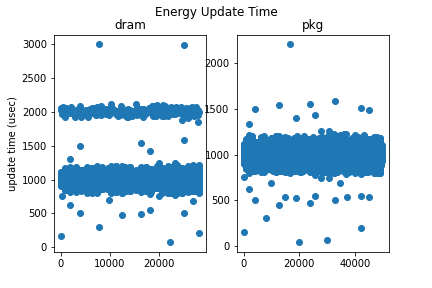
\includegraphics[width=10cm,height=10cm,keepaspectratio]{jmh/msr-update-rate/energy-update-time-simple.png}
    \caption{Energy Update Time (microseconds)}
    \label{fig:PKG-rapl-counter}
\end{figure}

% \begin{tabular}{lr}
\toprule
{} &          dram \\
\midrule
count &  28266.000000 \\
mean  &   1011.747860 \\
std   &    106.390894 \\
min   &     74.000000 \\
25\%   &    974.000000 \\
50\%   &   1000.000000 \\
75\%   &   1035.000000 \\
max   &   3070.000000 \\
\bottomrule
\end{tabular}

% \begin{tabular}{lr}
\toprule
{} &        dram.1 \\
\midrule
count &  49229.000000 \\
mean  &   1012.362896 \\
std   &    108.137976 \\
min   &     24.000000 \\
25\%   &    975.000000 \\
50\%   &   1000.000000 \\
75\%   &   1034.000000 \\
max   &   3031.000000 \\
\bottomrule
\end{tabular}

% \begin{tabular}{lr}
\toprule
{} &           pkg \\
\midrule
count &  49688.000000 \\
mean  &   1003.008694 \\
std   &     47.508242 \\
min   &     47.000000 \\
25\%   &    974.000000 \\
50\%   &   1000.000000 \\
75\%   &   1034.000000 \\
max   &   2198.000000 \\
\bottomrule
\end{tabular}

% \begin{tabular}{lr}
\toprule
{} &         pkg.1 \\
\midrule
count &  49689.000000 \\
mean  &   1002.989575 \\
std   &     47.588151 \\
min   &     24.000000 \\
25\%   &    974.000000 \\
50\%   &   1000.000000 \\
75\%   &   1033.000000 \\
max   &   1942.000000 \\
\bottomrule
\end{tabular}


These experiments confirm the expectation that the MSRs have a 1ms update rate, so all future sampling will happen at a 1ms rate, at minimum. 

Also worth noting that MSRs close off after several thousand repeated read attempts with no buffer time. \anote{What I meant by this: If you read the MSR over and over and over again with little to no other work in between, the MSR file shuts down and doesn't let you read any more. We had to put busywaits in our benchmarks to ``cool it off". This could be worth mentioning in that it solidifies the point that not only are you wasting time by sampling as fast as possible and trying for sub-millisecond periods, it also might temporarily ``break" the register to do it too often.}